\documentclass[final]{beamer}
\mode<presentation>
{
 % \usetheme{collis} 
\usetheme{ANLARM}
}
\graphicspath{{figures/}}
\usepackage{natbib}

\usepackage{times}
\usepackage{amsmath,amssymb}
\usepackage[english]{babel}
\usepackage[latin1]{inputenc}
\usepackage[printwatermark]{xwatermark}
\usepackage[orientation=landscape,size=a0]{beamerposter}  % e.g. custom size poster
\usepackage{tikz}
\addtobeamertemplate{block begin}{\pgfsetfillopacity{0.8}}{\pgfsetfillopacity{1}}

\usebackgroundtemplate{
\tikz\node[opacity=0.5] {\includegraphics[height=\paperheight,width=\paperwidth]{figures/radar2.png}};}


\title{\huge Architectures for Rainfall Property Estimation From Polarimetric Radar}
\author[Collis et al.]{Scott Collis\textsuperscript{1} {\texttt{scollis@anl.gov}},
 Scott Giangrande\textsuperscript{2},
  Jonathan Helmus\textsuperscript{1}
   and Silke Troemel\textsuperscript{3}}
\institute[Argonne]{
1: Argonne National Laboratory Argonne, IL United States \\
2: Brookhaven National Laboratory, Upton, NY United States\\
3: Meteorologisches Institut der Universit{\"a}t Bonn, Bonn, Germany}
\date{\today}
\begin{document}
\begin{frame}{} 
 \begin{columns}[t]
    \begin{column}{.3\linewidth}
  \vfill
  %%%%%%%%%%%Intro Block %%%%%%%%%%%%%%%%%%%%%%%%
      \begin{block}{Introducton}
        \begin{columns}[t]
          \begin{column}{.5\linewidth}
          %%%%%%%%%%%%%%%Col 1: Text%%%%%%%%%%%%%%%%%%%%
        \begin{itemize}
        \item Numerical simulations of decadal climate are done at resolutions far courser than the natural scale of precipitation. 
                 To even have a chance of understanding future precipitation extremes we must reconcile the relation between the statistics of broad-scale
                 precipitation and high resolution observations. 
        \item To this end The Department of Energy's ARM Climate Research Facility operates a network of 5 and 3 cm scanning radar systems. 
        \item Fixed sites are at the Azores, Barrow on the North Slope of Alaska and a multi-scale heterogeneous network on the Southern Great Plains of Oklahoma.                             
         \end{itemize}
         \end{column}
          \begin{column}{.5\linewidth}
          %%%%%%%%%%%%%%%%Col 2: Figure%%%%%%%%%%%%%%%%%%%
           \vskip0ex
            \centering    
           \includegraphics[width=0.95\linewidth]{figures/sgp_layout.png}\\[1ex]            
          \end{column}
         \end{columns}
         \end{block}
         
         
        \begin{block}{Achieving insight with the community: The \textcolor{red}{Py}thon \textcolor{red}{A}RM \textcolor{red}{R}adar \textcolor{red}{T}oolkit}
                \begin{columns}[t]
                    \begin{column}{.6\linewidth}
                        \begin{itemize}
                            \item Weather radars are not a new invention, first academic mention in \citet{bent_radar_1943}.
                            \item Massive advances in computing and radar software has not kept up.
                            \item They Python ARM Radar Toolkit, Py-ART  is a data model driven architecture for interactively and 
                            offline processing of active remote sensing data. Open source and, using GitHub, community based.
                            \item Part of a larger growing international community of codes, see \citet{heistermann_emergence_2014}
                            \item Twenty four forks, eight active contributors from multiple agencies and nations. Broad user base. 
                             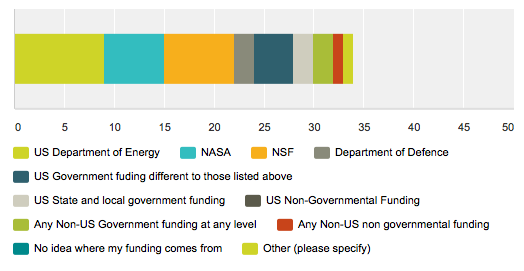
\includegraphics[width=0.8\linewidth]{figures/survey}\\[1ex]                        
                       \end{itemize}
                   \end{column}
                   \begin{column}{.4\linewidth}
                   \vskip0ex
                       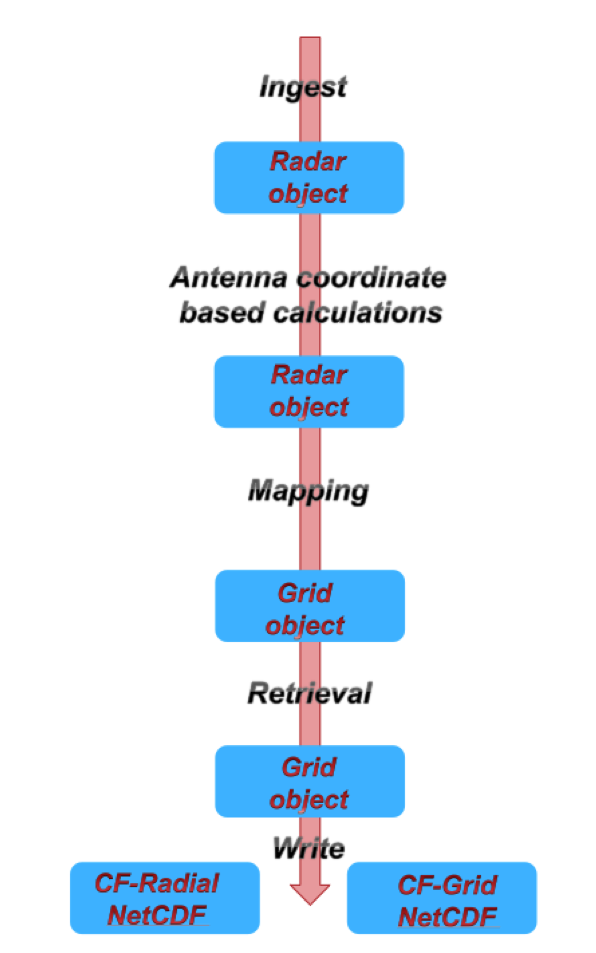
\includegraphics[width=0.9\linewidth]{figures/pyart-flow}\\[1ex]   
                   \end{column}
               \end{columns}
                       \end{block}
        
         \begin{block}{Links}
         	\begin{columns}[c]
         		\begin{column}{.3\linewidth}
		   		\\
         			The Python ARM Radar Toolkit :
         			{\small \hyperlink{http://arm-doe.github.io/pyart/}{http://arm-doe.github.io/pyart/}} 
         	
         		\end{column}
         		\begin{column}{.2\linewidth}
		                 \vskip0ex
		 		
\includegraphics[width=1\linewidth]{figures/pyart_qr}\\[1ex]   
        		 	\end{column}
			\begin{column}{.3\linewidth}
		   		\\
         			This is an open source poster, for notebooks, code and tex: 
         			{\small \hyperlink{http://github.com/scollis/AGU_2014_poster/}{http://github.com/scollis/AGU\_2014\_poster/}} 
         	
         		\end{column}
         		\begin{column}{.2\linewidth}
		                 \vskip0ex
		 		
\includegraphics[width=1\linewidth]{figures/git_repo_qr}\\[1ex]   
        		 	\end{column}
         	\end{columns}
         \end{block}

  		

    \end{column}
   %COL 2%
      \begin{column}{.3\linewidth}
  \vfill
 
     \begin{block}{Raw data to Quantitative Precipitation Estimates}
 	\begin{columns}[t]
		\begin{column}{.5\linewidth}
		\begin{itemize}
		\item Raw collected radar data in engineering units is unsuitable for comparison with model data. 
		\item Shorter wavelength radar have a higher attenuation cross section. However Signal to noise in phase information much higher and calibration insensitive.
		\item Measured phase is a mix of propagation phase, phase shift on backscatter and artifacts: {\tiny $\phi_{dp}^{signal}(r) = \phi_{dp}^{prop}(r) + \delta(r) + E(r)$}.
		\item When calculating Specific Differential Phase, {\small $K_{dp}$} only the propagation component should be considered, {\tiny $K_{dp} = \frac{d\phi_{dp}^{prop}(r)}{dr}$}.
		\item Method of \citet{giangrande_application_2013} used to extract {\small $\phi_{dp}^{prop}$} and a 20 point sobel filter 
		{\tiny$K_{dp} = \phi_{dp}^{prop} \ast f_{20} = \sum\limits_{M=0}^{19}   \phi_{dp}(r-M)f(M)$} where $f(M)$ is a linear ramp through zero. 
		\item Specific attenuation is calculated using {\small $K_{dp}$} and {\small $Z_e$} using a method after \citet{gu_polarimetric_2011} and is used as a an estimator for rainfall 
		using a method after \cite{ryzhkov_potential_2014}.
		\end{itemize}
		\end{column}
                \begin{column}{.5\linewidth}
                \begin{columns}[t]
                \begin{column}{.5\linewidth}
                		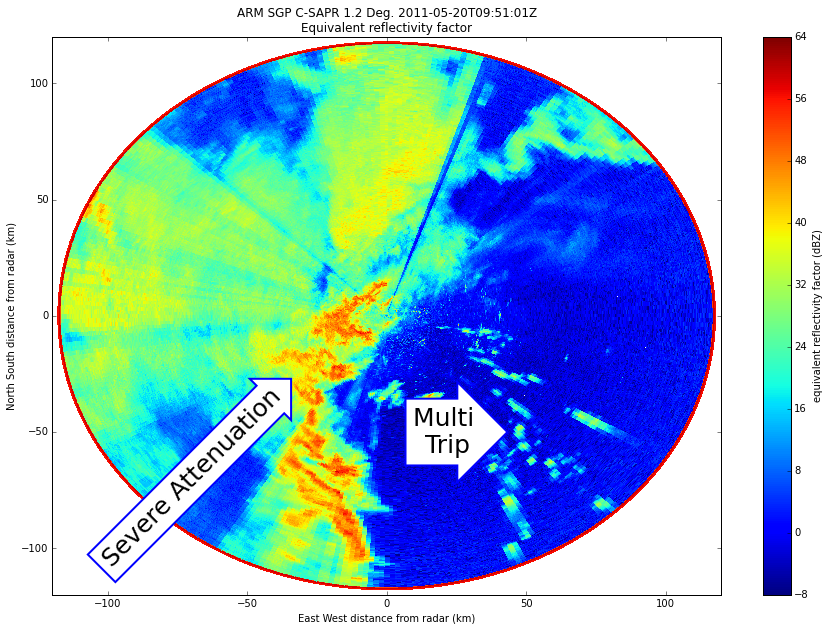
\includegraphics[width=1.0\linewidth]{figures/ze.png}\\[1ex]  %r1
           		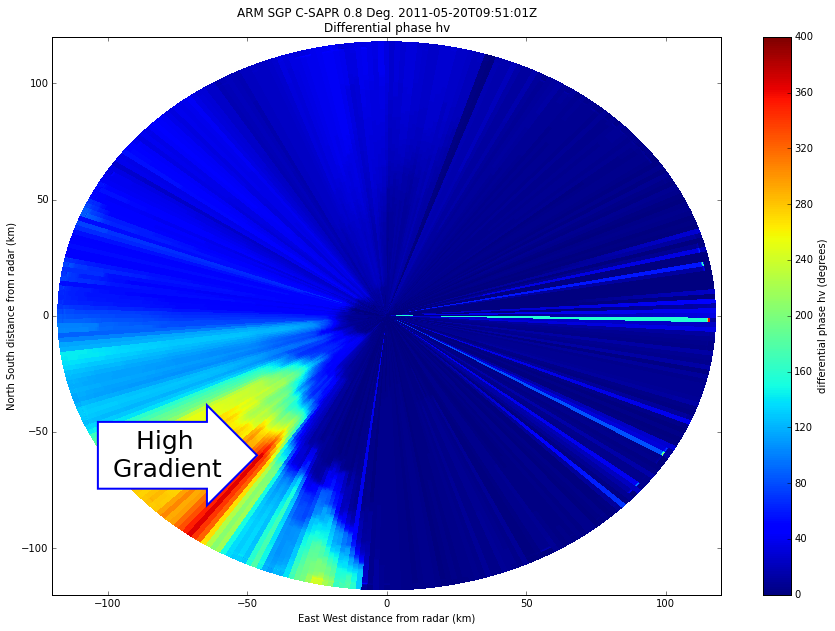
\includegraphics[width=1.0\linewidth]{figures/phidp_f.png}\\[1ex]   %r2 
			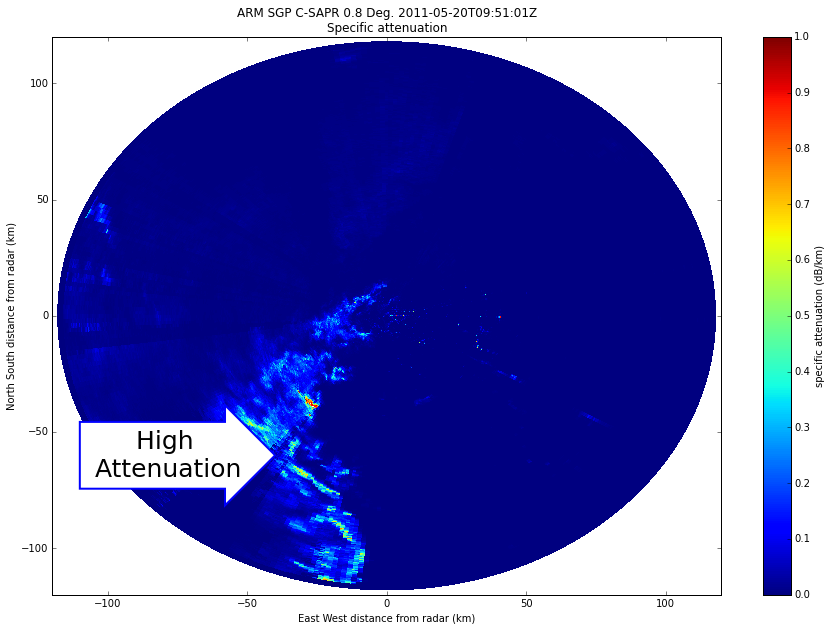
\includegraphics[width=1.0\linewidth]{figures/speca.png}\\[1ex]  
		\end{column}
		 \begin{column}{.5\linewidth}
                		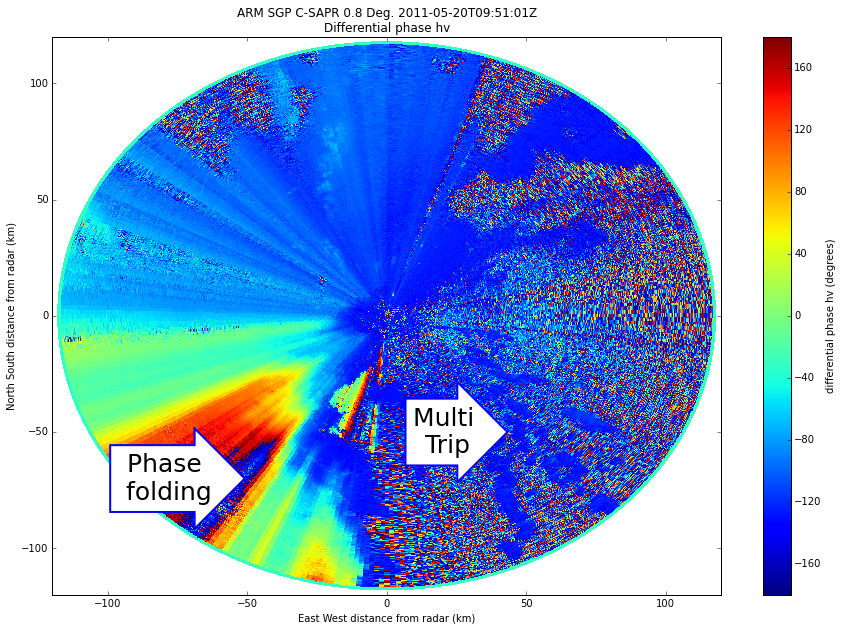
\includegraphics[width=1.0\linewidth]{figures/phidp.png}\\[1ex] %r1
           		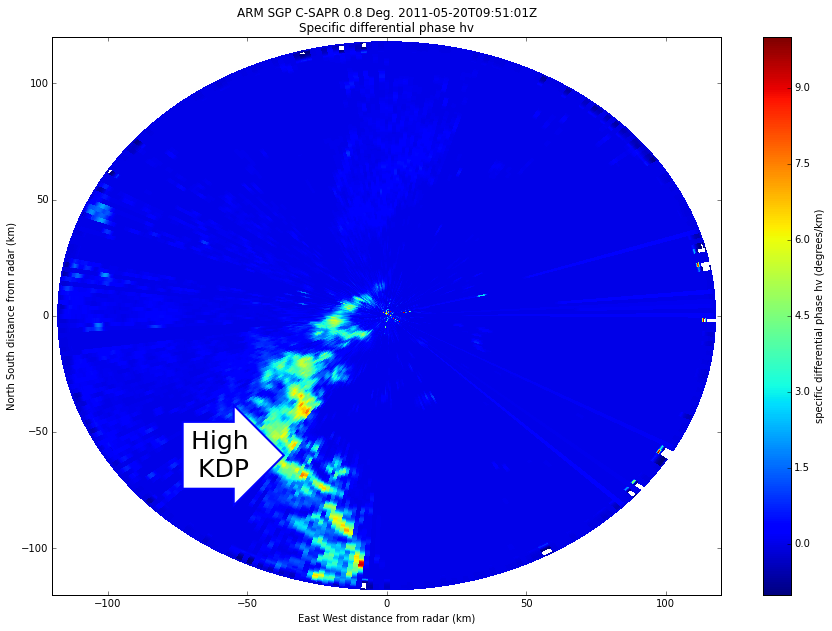
\includegraphics[width=1.0\linewidth]{figures/kdp.png}\\[1ex]    %r2
			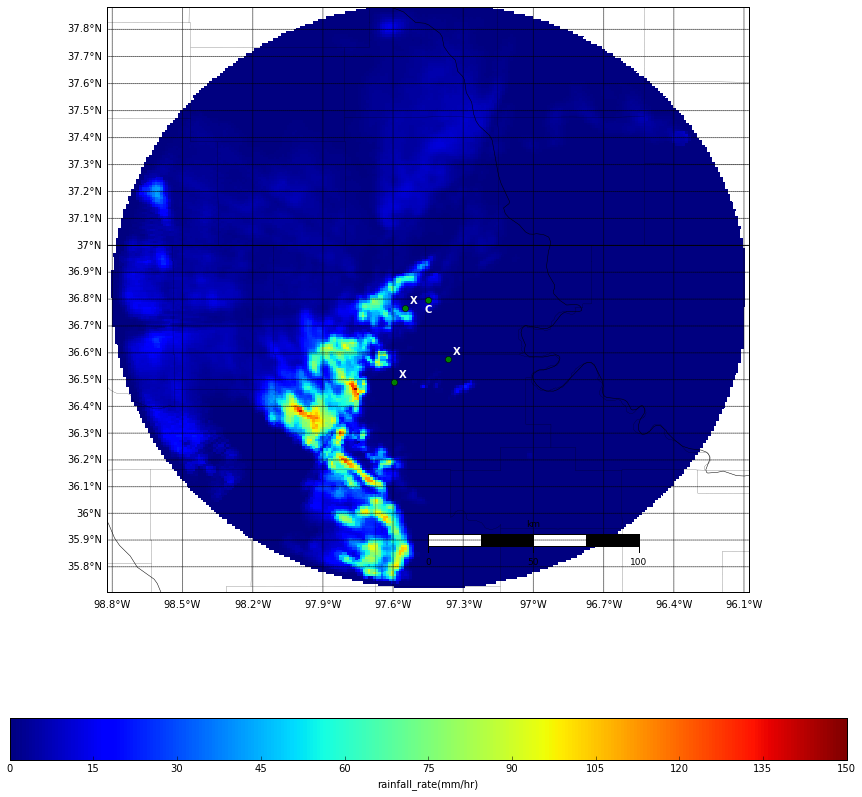
\includegraphics[width=1.0\linewidth]{figures/qpe.png}\\[1ex]  
		
		\end{column}
		\end{columns}
 		\end{column}
	\end{columns}
      \end{block}
       \begin{block}{Mapping: Objective analysis}
         \end{block}


    \end{column}
%COL 3%
  \begin{column}{.3\linewidth}
  \vfill
   \begin{block}{Advective interpolation}
 	\begin{columns}[t]
		\begin{column}{.5\linewidth}
		\end{column}
                \begin{column}{.5\linewidth}
           		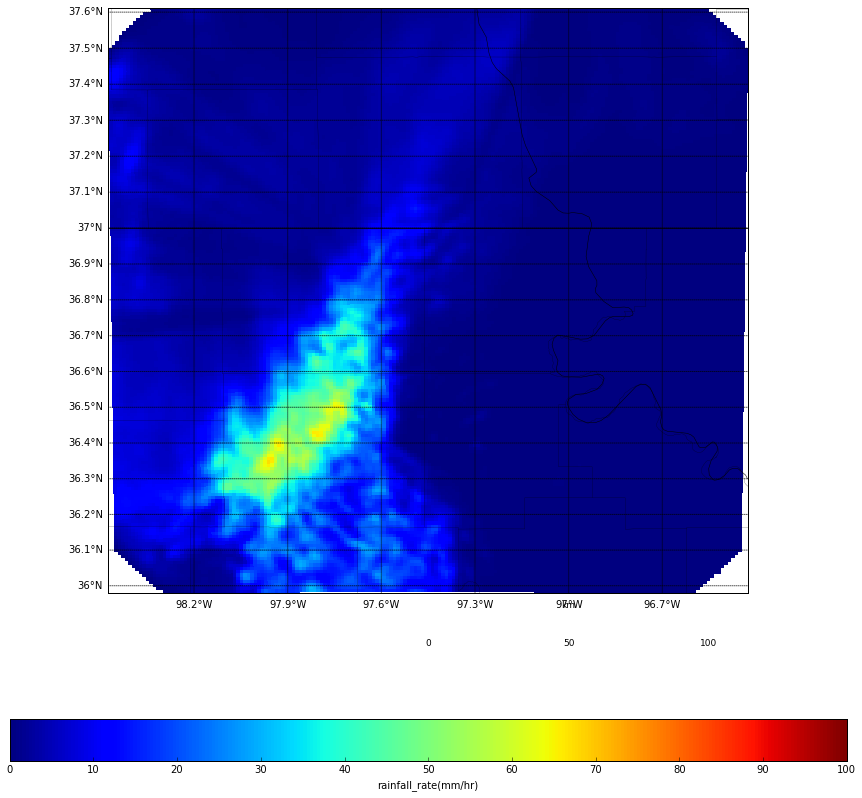
\includegraphics[width=1.0\linewidth]{figures/basic_accumulation.png}\\[1ex]     
            		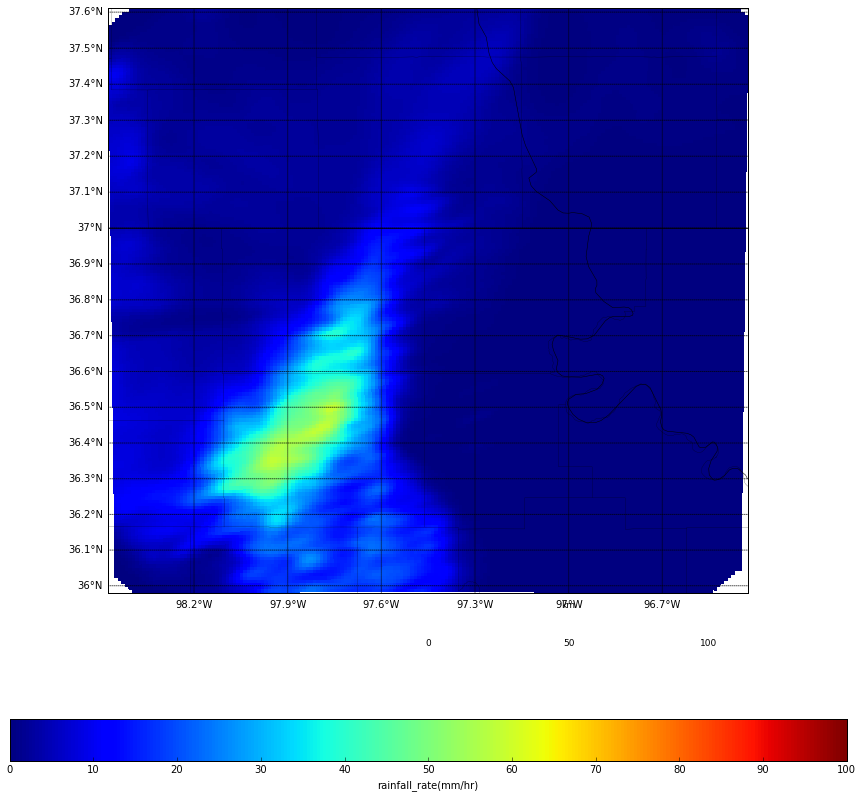
\includegraphics[width=1.0\linewidth]{figures/advective_accum.png}\\[1ex]  
 		\end{column}
	\end{columns}
      \end{block}
   
   
        \begin{block}{References}
        \small
       \bibliographystyle{ametsoc}
       \bibliography{zotero} 
         \end{block}


    \end{column}

  \end{columns}


  \vfill
\end{frame}
\end{document}


%%%%%%%%%%%%%%%%%%%%%%%%%%%%%%%%%%%%%%%%%%%%%%%%%%%%%%%%%%%%%%%%%%%%%%%%%%%%%%%%%%%%%%%%%%%%%%%%%%%%
%%% Local Variables: 
%%% mode: latex
%%% TeX-PDF-mode: t